%&pdflatex

\documentclass[12pt]{report}

\usepackage{algorithm}
\usepackage{algpseudocode}
\usepackage{amsmath} % for implementation of the matrix environment
\usepackage{blindtext}
\usepackage{caption}
\usepackage{color}
\usepackage[pdftex]{graphicx} \graphicspath{{./plots/}}
\usepackage{epstopdf} \epstopdfsetup{update} % only regenerate pdf files when eps file is newer
\usepackage{float} % figure groups aka floats
\usepackage{forest} % for MFS elimination tree diagram
\usepackage[left=3.5cm, right=2.5cm]{geometry} % margins
\usepackage[shellescape,latex]{gmp} % metapost for UMLs
\usepackage[hidelinks]{hyperref} % ToC/LoA/LoF/LoT entries are links
\usepackage{mathptmx} % Times New Roman like font
\usepackage{pdfpages} % for inserting pdf as the initial pages
\usepackage{setspace} \onehalfspacing % 1.5 line spacing
\usepackage{subcaption}
\usepackage{xfrac} % nice slanted fractions

\captionsetup[figure]{labelfont={bf}, textfont={small}}
\captionsetup[subfigure]{labelfont={bf}, textfont={small}}

\newcommand{\bt}{\blindtext}
\newcommand{\eps}{\varepsilon}
%\newcommand{\rev}[1]{\textcolor{red}{#1}}
\newcommand{\rev}[1]{#1}
\newcommand{\T}[1]{\texttt{#1}}

\algnewcommand\And{\,\textbf{and}\,}
\algnewcommand\Or{\,\textbf{or}\,}
\algnewcommand{\LineComment}[1]{\State \(\triangleright\) #1}


\begin{document}


\includepdf[pages={-,{}}]{initial-pages.pdf} % `-' for all pages, `{}' for an empty page

\tableofcontents


\chapter{Preface}

\section{Motivation}

\bt

\section{Content of this work}

\bt

The chapter \ref{chap:problem-formulation} provides the requirements for the project,
and as well formulates the sample problem of shallow water simulation.
The chapter \ref{chap:methodology} outlines the tools and methods necessary for approaching the problems.
In the chapter \ref{chap:docs} I thoroughly document the software I developed to accomplish the research goals.
I discuss the obtained results in the chapter \ref{chap:evaluation} and sum up the thesis in chapter \ref{chap:conclusions}.


\section{State of the art}

\subsection{Technology 1}

A lot of bibliography citations here...

\bt

\subsection{Technology 2}

\bt

\section{Main thesis of this work}

The main thesis of this work may be expressed as follows:

\medskip

\textit{
	\bt
}



\chapter{Problem formulation} \label{chap:problem-formulation}

Describe what each section contains...

\section{Issues to be addressed in this work}

\subsection{(e.g.) Algorithmic challenges}

\bt

\subsection{(e.g.) Parallelization challenges}

\bt

\section{Functional requirements}

\begin{enumerate}
	\item Core functionalities
	\begin{enumerate}
		\item ...
		\item ...
		\item ...
	\end{enumerate}

	\item Adaptation strategies
	\begin{enumerate}
		\item ...
		\item ...
	\end{enumerate}

	\item Visualization and profiling
	\begin{enumerate}
		\item ...
		\item ...
		\item ...
		\item ...
	\end{enumerate}
\end{enumerate}


\section{Non-functional requirements}

\begin{enumerate}
	\item Performance and complexity
	\begin{enumerate}
		\item ...
		\item ...
		\item ...
	\end{enumerate}

	\item Development requirements
	\begin{enumerate}
		\item ...
		\item ...
	\end{enumerate}
\end{enumerate}




\chapter{Solution methodology} \label{chap:methodology}

\bt

\section{Method 1}

\bt

\section{Method 2}

\bt 

\section{Method 3}

Some nice matrices...

\begin{equation}
	A = \begin{bmatrix}
		1 &    &    &    &    &    &    & \\
		1 & -2 &  1 &    &    &    &    & \\
		  &  1 & -2 &  1 &    &    &    & \\
		  &    &  1 & -2 &  1 &    &    & \\
		  &    &    &  1 & -2 &  1 &    & \\
		  &    &    &    &  1 & -2 &  1 & \\
		  &    &    &    &    &    &  1 & \\
	\end{bmatrix}
	\hspace{1cm}
	B = \begin{bmatrix}
		0 \\
		4 \\
		4 \\
		4 \\
		4 \\
		4 \\
		0
	\end{bmatrix}
\end{equation}

Some nice diagrams...

\newcommand{\cv}[1]{ % column vector
	$\begin{bmatrix} #1 \end{bmatrix}$
}
\newcommand{\Cv}[1]{ { \cv{#1} } } % shortcut for tree leaves
\newcommand{\elim} { $\xrightarrow{E}$ }
\newcommand{\merge} { $\xrightarrow{M}$ }
\newcommand{\xtract} { $\xrightarrow{X}$ }

\begin{figure}[H]
	\centering
	\caption{Elimination tree for multifrontal solver}
	\label{fig:mfs-elim-tree}
	\begin{forest}
		for tree = {
			draw,
			edge={<-, line width=2pt},
			minimum height=2cm,
			anchor=north,
			align=center,
			child anchor=north
		},
		[ { \merge \cv{x_1 \\ x_5 \\ x_7} \elim \cv{x_1 \\ x_7 } }
			[ { \merge \cv{x_1 \\ x_3 \\ x_5} \elim \cv{x_1 \\ x_5} }
				[ { \merge \cv{x_1 \\ x_2 \\ x_3} \elim \cv{x_1 \\ x_3} }
					[ \Cv{x_1 \\ x_2} ]
					[ \Cv{x_2 \\ x_3} ]
				]
				[ { \merge \cv{x_3 \\ x_4 \\ x_5} \elim \cv{x_3 \\ x_5} }
					[ \Cv{x_3 \\ x_4} ]
					[ \Cv{x_4 \\ x_5} ]
				]
			]
			[ { \merge \cv{x_5 \\ x_6 \\ x_7} \elim \cv{x_5 \\ x_7} }
				[ \Cv{x_5 \\ x_6} ]
				[ \Cv{x_6 \\ x_7} ]
			]
		]
	\end{forest}
\end{figure}

\pagebreak

Some nice algorithms...

\newcommand{\U}{\mathcal{U}}

\begin{algorithm}
\caption{One iteration of the double-grid algorithm}
\label{alg:two-grid}

\begin{algorithmic}

	\State Compute the solution $\U^C$ on the coarse mesh
	\State Split each element of the coarse mesh, thus obtaining the fine mesh
	\State Compute the solution $\U^F$ on the fine mesh

	\For{\textbf{each} coarse mesh element $\eps_i$}
		\LineComment{$\rho_i$ is the relative error}
		\State $ \rho_i \gets \left|
				\frac {
					\U^F_i - \U^C_i
				} {
					\U^F_i
				}
			\right| $
	\EndFor

	\State $\rho_{max} \gets$ $max_i(\rho_i)$

	\For{\textbf{each} element $\eps_i$}
		\If {$ \rho_i > \tau \cdot \rho_{max} $}
			\State adapt the $\eps_i$ element (split into two halves)
		\EndIf
	\EndFor

\end{algorithmic}
\end{algorithm}

\pagebreak

Some nice figures...

\begin{figure}[H]
	\centering

	\caption[Double-grid h-adaptation strategy, steps 1-2] {
		Steps 1-5 of the double-grid h-adaptation strategy, quadratic B-splines
	}
	\label{fig:h-adapt-two-grid}

	\begin{subfigure}[h]{1.0\textwidth}
		\centering
		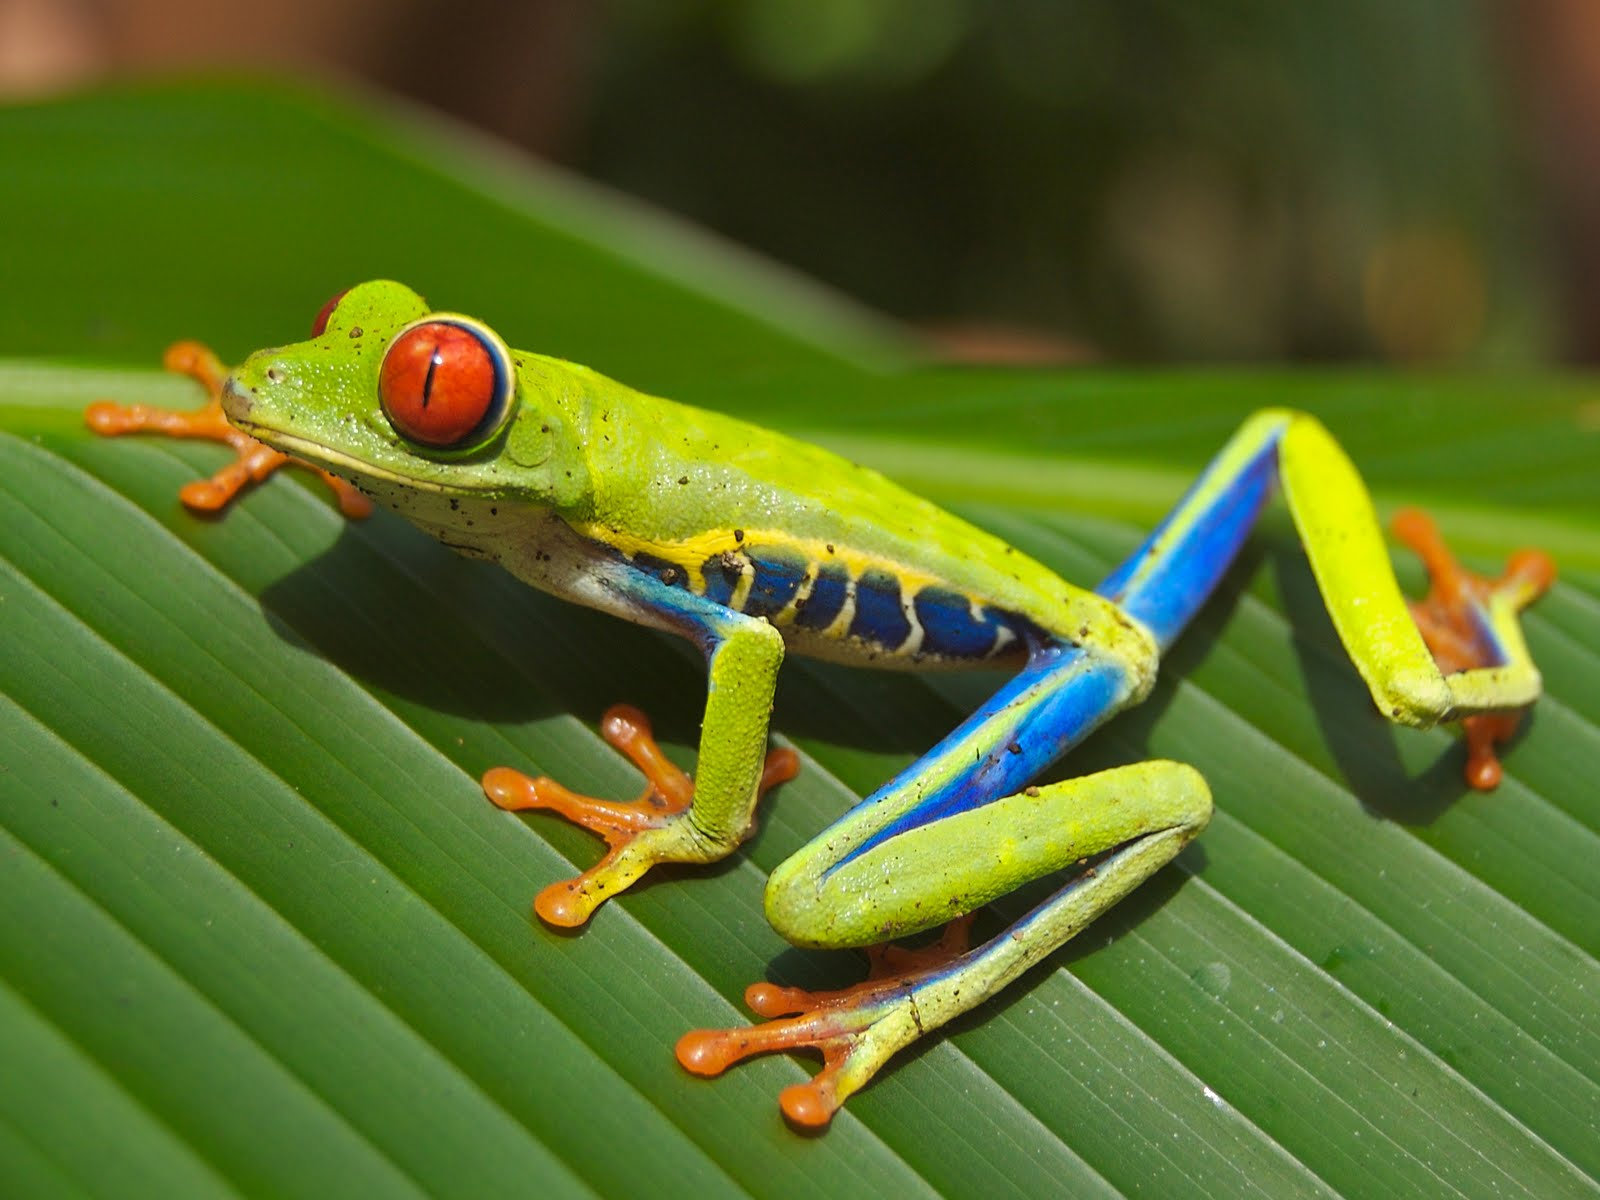
\includegraphics[scale=0.2]{frog.jpg}
		\caption{
			Step 1.
			A solution is delivered on coarse (4 elements) and fine grid (8 elements).
			Red line marks the coarse-grid solution, green line --- the fine-grid solution and black line --- the exact (analytic) solution.
		}
		\label{fig:h-adapt-two-grid-1}
	\end{subfigure}

	\begin{subfigure}[h]{1.0\textwidth}
		\centering
		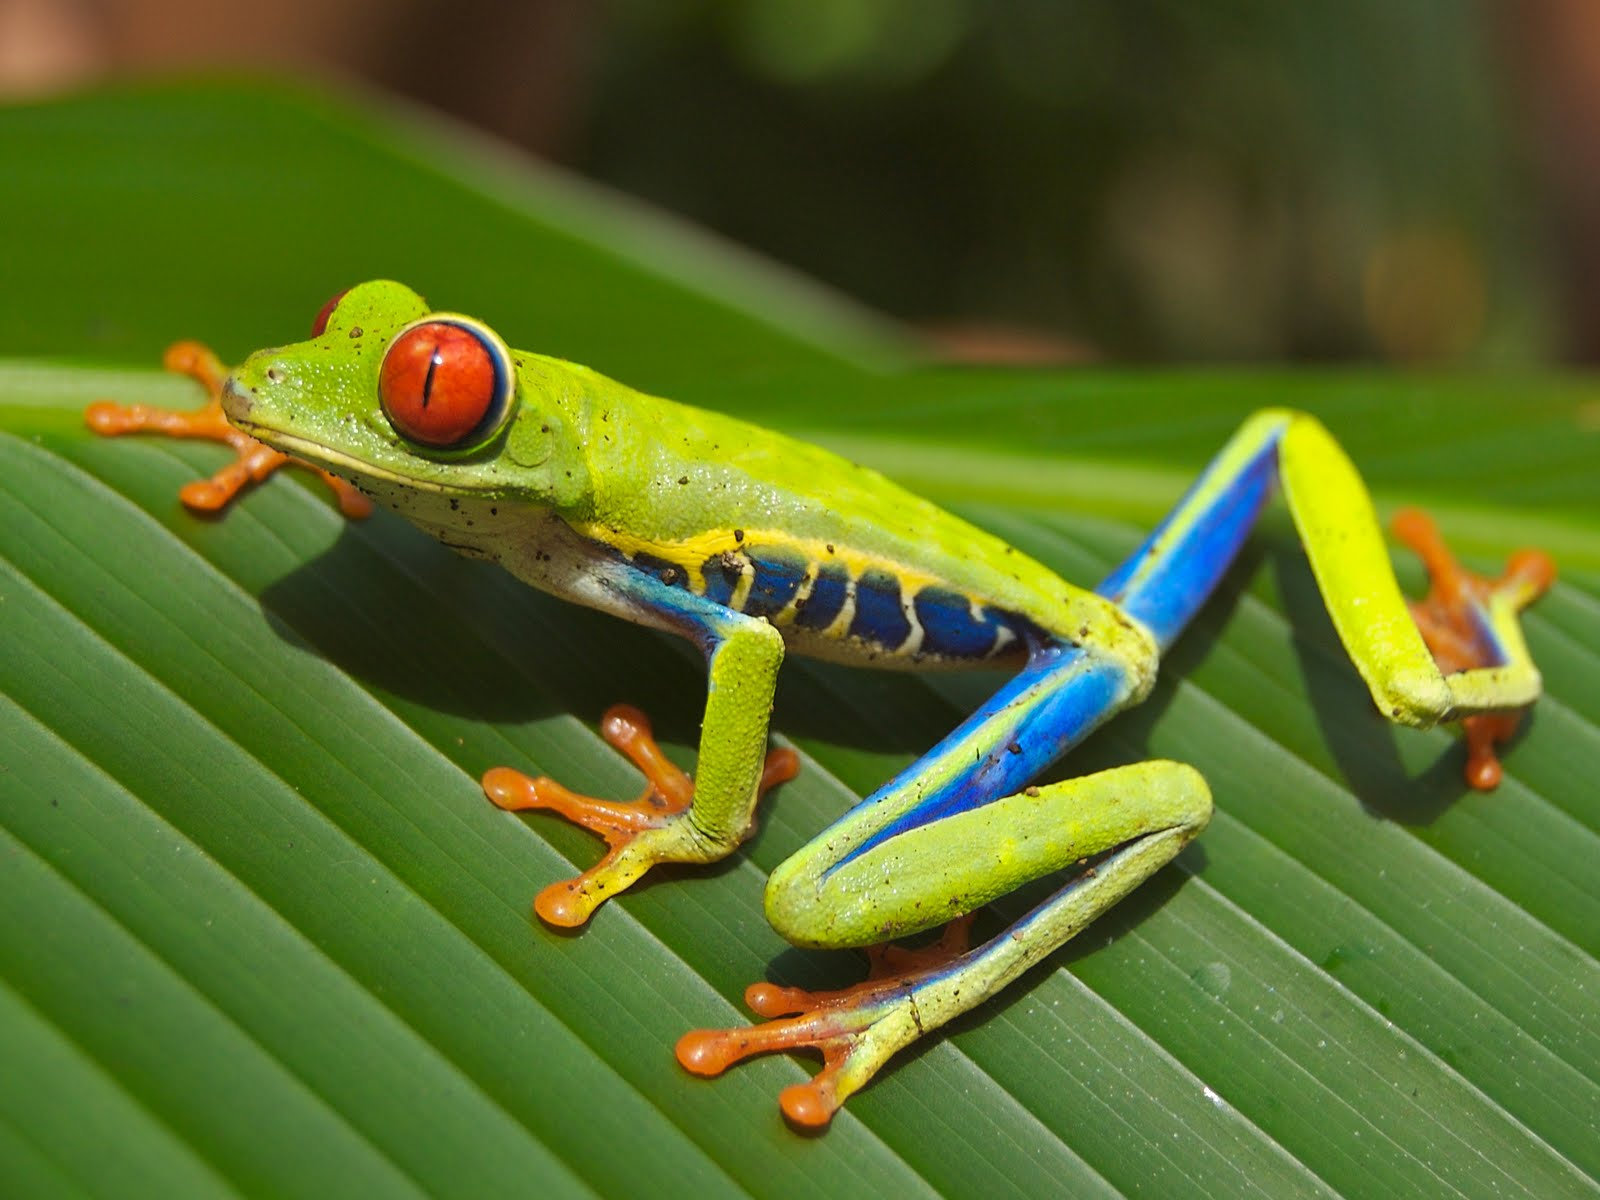
\includegraphics[scale=0.2]{frog.jpg}
		\caption{
			Step 2.
			Since the maximal error multiplied by $\tau$ (here set to 20\%) were lower than the error on any element,
			the algorithm halved all four elements after step 1.
		}
		\label{fig:h-adapt-two-grid-2}
	\end{subfigure}
\end{figure}


\begin{figure}[H]
	\ContinuedFloat % continue from previous page
	\caption[Double-grid h-adaptation strategy, steps 3-4]{} % for subcaption package to ensure proper numbering

	\begin{subfigure}[h]{1.0\textwidth}
		\centering
		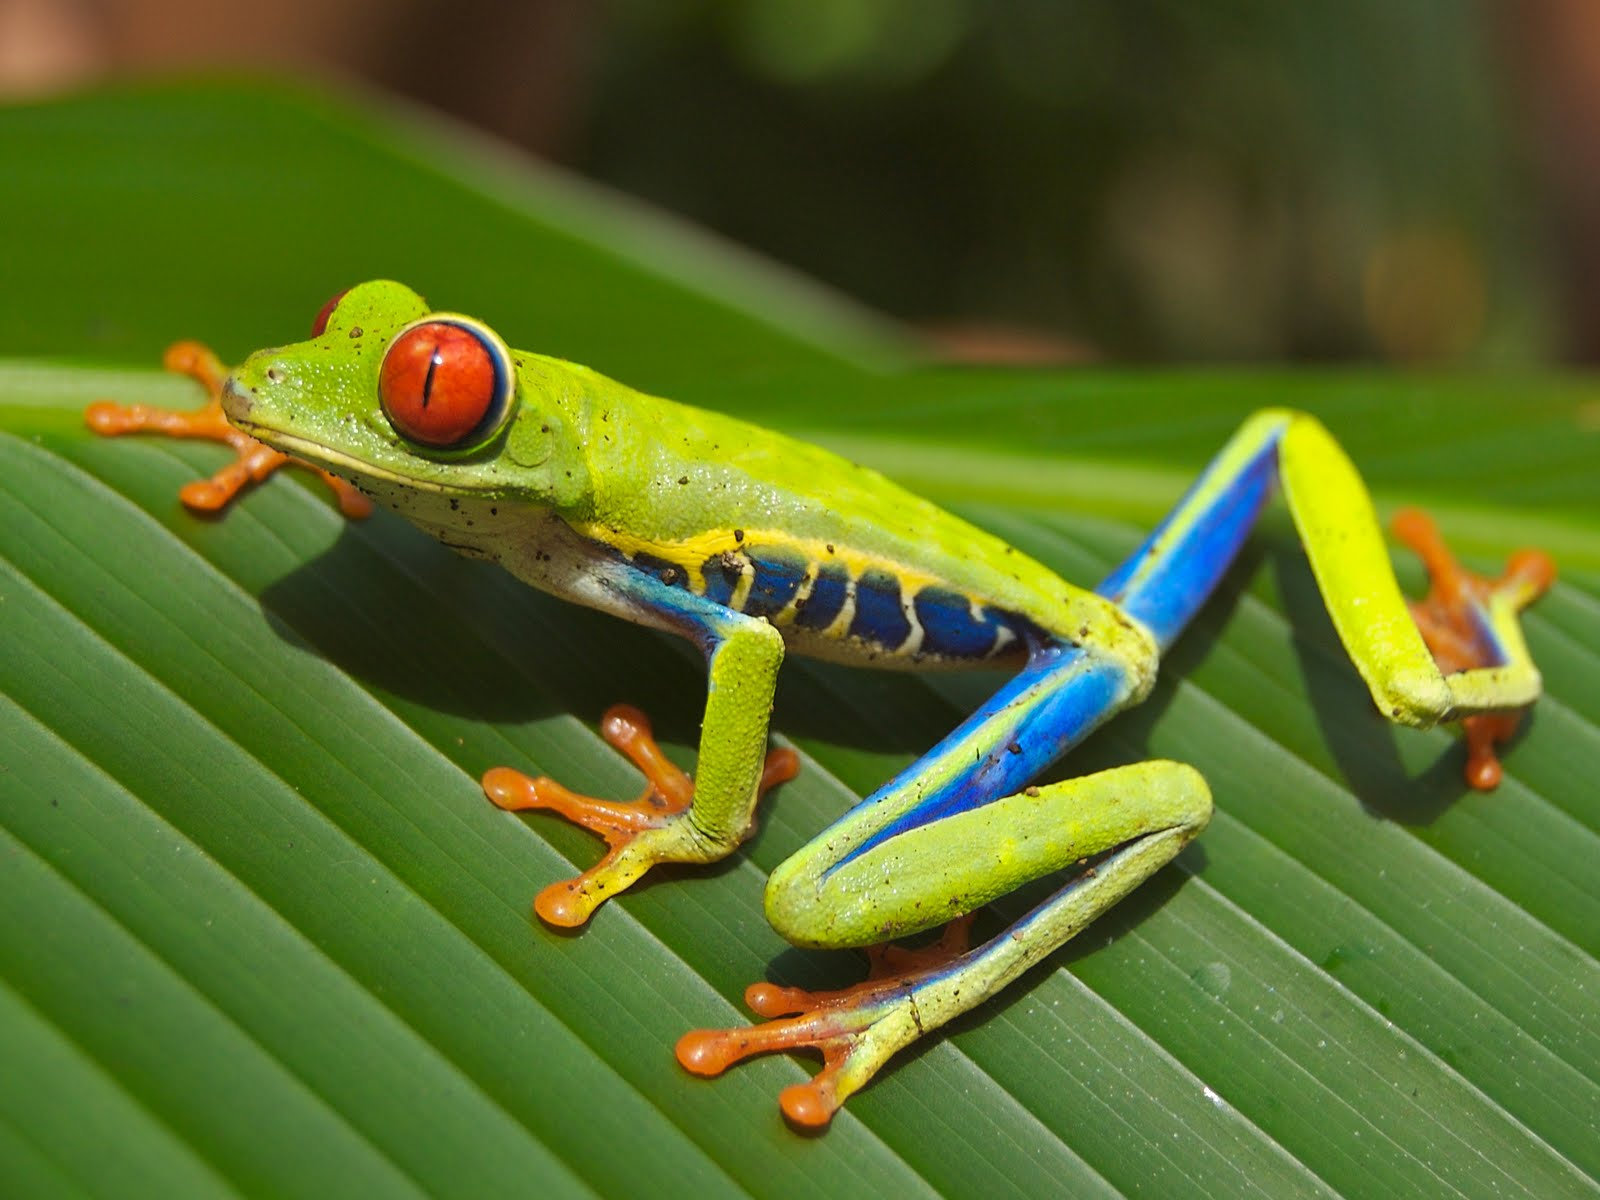
\includegraphics[scale=0.2]{frog.jpg}
		\caption{
			Step 3.
			The extreme left and right elements did not get refined after the step 2.
		}
		\label{fig:h-adapt-two-grid-3}
	\end{subfigure}

	\begin{subfigure}[h]{1.0\textwidth}
		\centering
		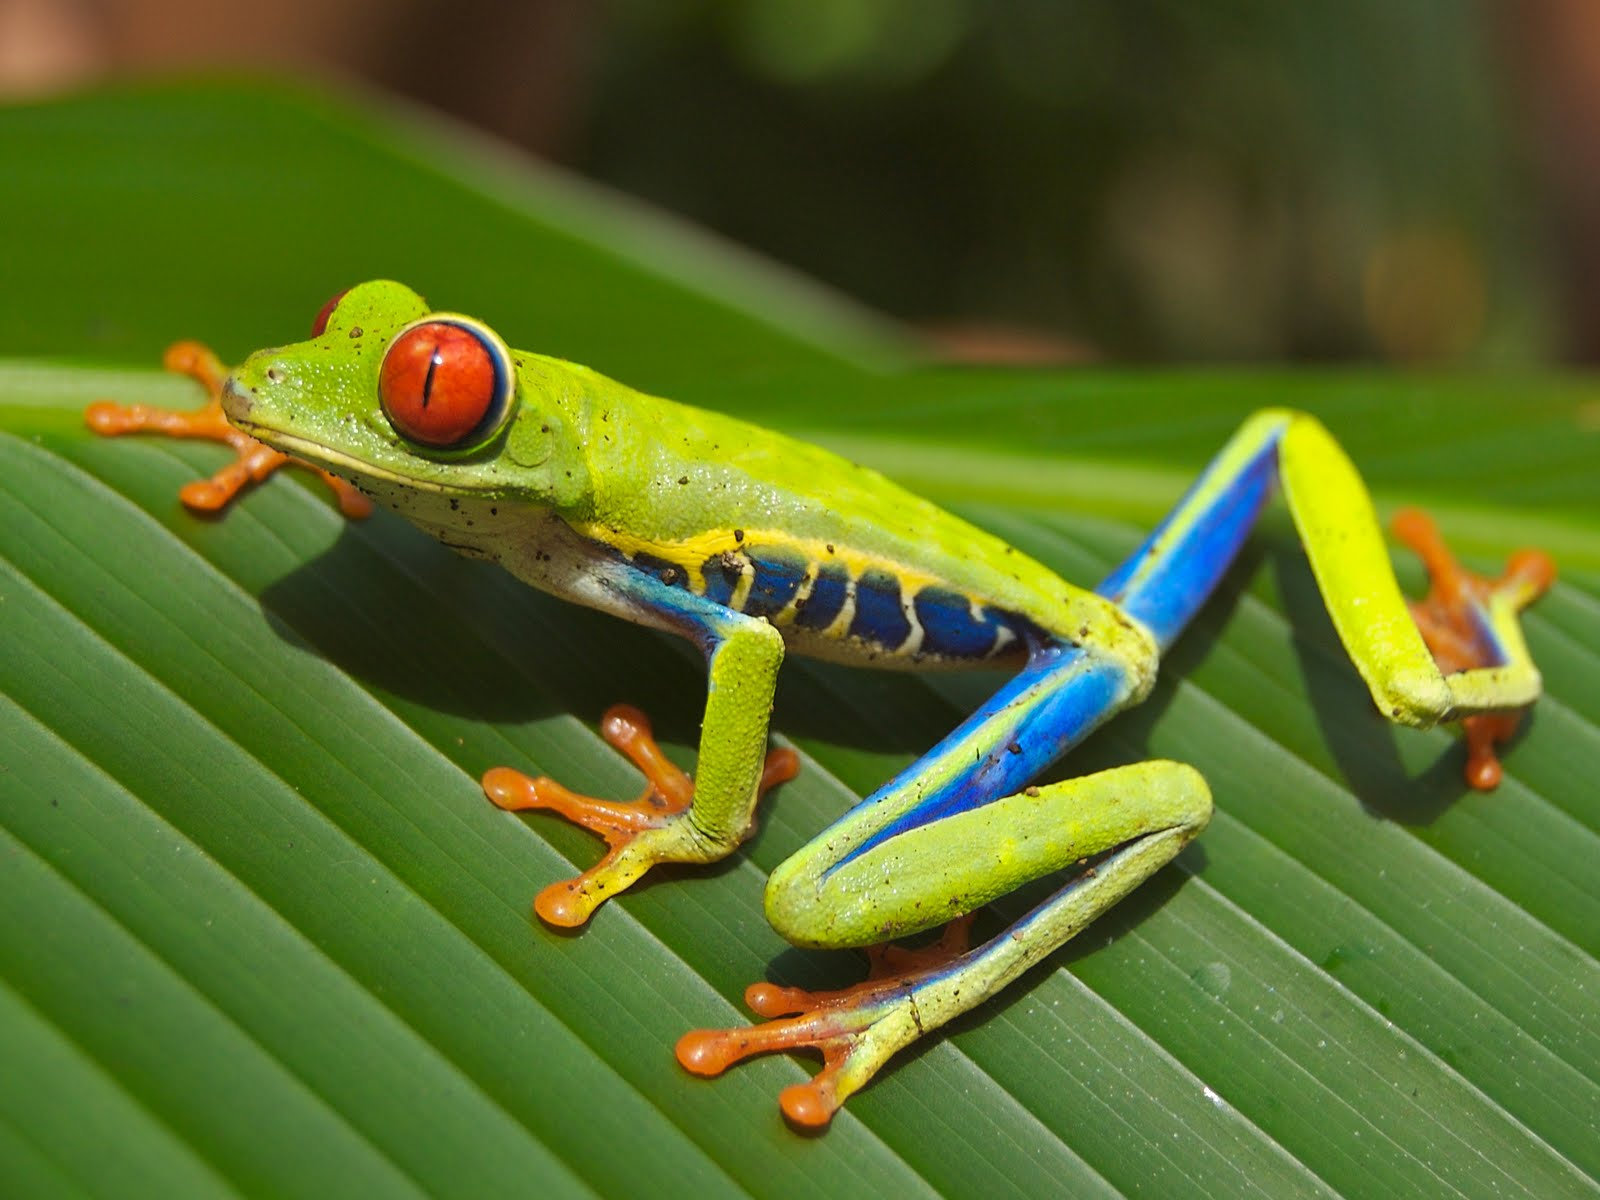
\includegraphics[scale=0.2]{frog.jpg}
		\caption{
			Step 4
		}
		\label{fig:h-adapt-two-grid-4}
	\end{subfigure}
\end{figure}




\chapter{Project documentation} \label{chap:docs}

\newcommand{\uml}[2] {
	\begin{figure}[H]
		\centering
		\caption{#1}
		\begin{mpost}[mpsettings=input metauml;]
			#2
		\end{mpost}
	\end{figure}
}

\bt

\section{Some clever stuff} \label{sec:cuda}

\bt

\section{API components overview} \label{sec:api-overview}

Nice UML no. 1...

\uml{IsogeometricFEM class} {
	Class.C("IsogeometricFEM") ()
		("+ apply(pde: PDE, bcs: BoundaryConditions,
			base: BsplineBase, solver: Solver, femConfig: FEMConfig)");
	drawObject(C);
}

Nice UML no. 2...

\uml{HAdaptiveIsogeometricFEM interface} {
	Interface.I("HAdaptiveIsogeometricFEM")
		("+ apply(pde: PDE, bcs: BoundaryConditions,
			adaptationThreshold: Double, solver: Solver, femConfig: FEMConfig)");
	classStereotypes.I("<<interface>>");
	drawObject(I);
}


\section{Detailed API specification and class diagrams} \label{sec:api-detail}

And another large UML...

\uml{The overall class diagram} {
	Class.IsogeometricFEM("IsogeometricFEM")
		() ("+ apply(...)");

	Class.PDE("PDE")
		("+ lhsCoefs: Function[1..*]", "+ rhs: Function") ();
	IsogeometricFEM.n = PDE.s + (60, -60);

	Class.BoundaryConditions("BoundaryConditions")
		("+ left: Double", "+ right: Double",
		 "+ leftType: BoundaryType", "+ rightType: BoundaryType") ();
	IsogeometricFEM.s = BoundaryConditions.n + (60, 60);

	Interface.Base("Base")
		("+ count(): Int",
		 "+ eval(...): Double",
		 "+ getSupport(no: Int): Range");
	classStereotypes.Base("<<interface>>");
	IsogeometricFEM.w = BsplineBase.e + (-150, 0);

	AbstractClass.GriddedBase("GriddedBase") ()
		("+ getGrid(): PointSequence",
		 "+ getGridSpan(index: Int): IntRange",
		 "+ getSupport(no: Int): Range");
	Base.n = GriddedBase.s + (-80, -60);

	Class.BsplineBase("BsplineBase") ()
		("+ getGrid(): PointSequence",
		 "+ getGridSpan(index: Int): IntRange",
		 "+ getSupport(no: Int): Range");
	Base.n = BsplineBase.s + (80, -60);

	Interface.Solver("Solver")
		("+ apply(...)");
	classStereotypes.Solver("<<interface>>");
	IsogeometricFEM.s = Solver.n + (-60, 60);

	Class.GaussSolver("GaussSolver")
		() ("+ apply(...)");
	Solver.e = GaussSolver.w + (-60, 0);

	Class.MultifrontalSolver("MultifrontalSolver")
		() ("+ apply(...)");
	Solver.s = MultifrontalSolver.n + (0, 60);


	drawObjects(
		IsogeometricFEM,
		PDE, BoundaryConditions,
		Base, GriddedBase, BsplineBase,
		Solver, GaussSolver, MultifrontalSolver
	);

	link(dependency)(IsogeometricFEM.n -- PDE.s);
	link(dependency)(IsogeometricFEM.n -- BsplineBase.s);
	link(dependency)(IsogeometricFEM.s -- BoundaryConditions.n);
	link(dependency)(IsogeometricFEM.s -- Solver.n);
	link(realization)(GriddedBase.s -- Base.n);
	link(realization)(BsplineBase.s -- Base.n);
	link(realization)(GaussSolver.w -- Solver.e);
	link(realization)(MultifrontalSolver.n -- Solver.s);
}



\chapter{Evaluation of the results} \label{chap:evaluation}

\bt

\section{e.g. Convergence analysis} \label{sec:convergence}

\bt

\section{e.g. Complexity analysis} \label{sec:complexity}

\bt

\section{e.g. Flood simulation results} \label{sec:flood-results}

\bt


\chapter{Conclusions and future works} \label{chap:conclusions}

\section{Achieved goals and observations}

\bt 

\section{Areas for development}

\bt



\cleardoublepage % to ensure that the page reference is correct
\addcontentsline{toc}{chapter}{\listfigurename}
\listoffigures

\begingroup
	\let \clearpage \relax % to suppress page break

	\cleardoublepage
	\addcontentsline{toc}{chapter}{\listalgorithmname}
	\listofalgorithms
\endgroup

\nocite{*} % forces bibtex to include all citations, whether or not they were referred to in the paper

\cleardoublepage
\addcontentsline{toc}{chapter}{Bibliography}
\bibliographystyle{bib-style}
\bibliography{bibliography}

\end{document}

